% !TeX root = ../main.tex
\section{Methodology}
\label{sec:methodology}
The methodology will be focussed into three parts; the training of initial models, the compression of these models, and the creation and optimisation of a full-stack system to utilise these models to apply high-level analysis of broadcast soccer film. 


\subsection{Model Training Procedure}
\label{subsec:training}

To support fair comparison, all uncompressed object detection and keypoint detection models were trained under a standard procedure. Training was initialised from COCO-pretrained weights \cite{lin2015microsoftcococommonobjects}, and then fine-tuned on a football-targeted dataset. All models were trained in PyTorch and saved as \verb|.pt| checkpoints prior to compression. Training used an input resolution of $1280 \times 1280$, a batch size of 32, and was conducted on the UCD high-performance cluster \textit{UCDSonic}. Optimisation used stochastic gradient descent with an initial learning rate of 0.01, momentum 0.937, and weight decay $5\times10^{-4}$ \cite{ultralytics_cfg}. Training ran for up to 500 epochs, with a 3-epoch warm-up schedule and early stopping patience of 60 epochs.

An initial benchmarking study was performed to identify the most suitable model family for the remainder of the work, based on analytical performance and hardware usage. A separate preliminary study was then conducted to determine the most suitable dataset for the full object detection study, in which 10 model variants were trained under identical conditions and evaluated across three labelled football broadcast datasets: SoccerNet \cite{tracking}, Roboflow \cite{roboflow_sports_repo}, and Football Analytics \cite{roboflow_football_analytics_gnykk_model1}. For pitch keypoint detection, the Roboflow football field dataset \cite{roboflow_football_field_detection_f07vi_dataset15} was used throughout.

\subsection{Compression}

As discussed in the Literature Review, three chief compression techniques have been explored: quantisation, knowledge distillation, and pruning. Figure \ref{fig:compressionplan} below displays the various combinations of compression techniques applied. 

\begin{figure}[H]
  \centering
  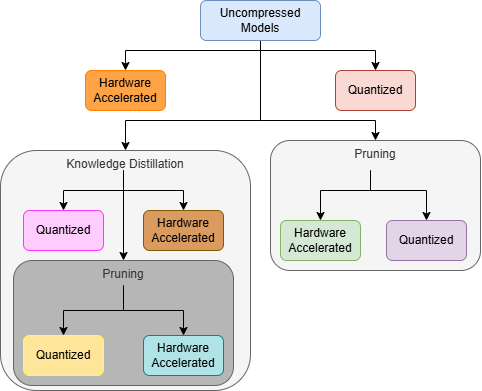
\includegraphics[width=.7\textwidth]{images/compression.png}
  \caption{Proposed full-stack system diagram.}
  \label{fig:compressionplan}
\end{figure}


In total, 11 compression configurations are applied to the baseline uncompressed models. These comprise the four individual techniques—hardware acceleration, quantisation, knowledge distillation, and pruning—together with seven hybrid configurations formed by combining these methods in different ways.
\subsection{Hardware Acceleration}
After training in PyTorch, each model checkpoint was exported from its native \texttt{.pt} format to a TensorRT \texttt{.engine} file in FP32 precision to enable hardware-accelerated inference on the NVIDIA Jetson Orin Nano. This export stage was included so that evaluation could be performed using the deployment runtime intended for the target edge device, rather than relying on the original training framework. While FP32 retains full numerical precision, conversion to TensorRT still enables substantial optimisation through techniques such as graph simplification, layer fusion, and improved kernel scheduling. This made FP32 engine export a suitable deployment format for measuring model performance under realistic edge inference conditions while avoiding changes to the underlying numerical representation.

This approach was used because it reduces inference overhead and improves deployment efficiency on embedded GPU platforms. NVIDIA recommends separating engine building from inference itself: the engine is built and serialized once, then loaded later for repeated inference runs. This avoids repeating the expensive optimization stage each time the application starts and allows TensorRT to exploit hardware-specific optimizations such as reduced-precision execution. A further practical consideration is that .engine files are generally tied to the TensorRT version and hardware platform on which they were created, meaning that engines usually need to be rebuilt if the deployment environment changes significantly.

\subsubsection{Quantisation}

FP16 and INT8 quantisation was implemented through post-training export of trained PyTorch checkpoints to TensorRT \texttt{.engine} files, enabling reduced-precision inference on the NVIDIA Jetson Orin Nano. Rather than modifying the model training stage, quantisation was applied at deployment time in order to reduce computational and memory requirements on the target edge device. All exports were performed at a fixed input resolution of 1280×1280 and with ONNX opset 20 to maintain consistency across models \cite{inbook, nvidia_modelopt}. This allowed quantisation to be evaluated as a practical deployment-stage compression technique for improving inference efficiency while preserving acceptable model performance.

For INT8 engine generation, calibration data was provided during export to estimate representative activation ranges before deployment \cite{nvidia_modelopt}. Task-specific dataset definitions were used for object detection and pose estimation, with calibration samples drawn from the training split by default and optionally limited by dataset fraction. The resulting TensorRT engines were then evaluated through the same benchmarking and validation pipeline as the other deployed models, allowing their impact on latency, accuracy, and hardware usage to be assessed consistently on the Jetson Orin Nano.


\subsubsection{Pruning}
Pruning was implemented as structured channel pruning using NVIDIA ModelOpt FastNAS \cite{248452, nvidia_modelopt}. This approach searches for a reduced channel configuration under an explicit FLOP constraint, producing smaller and more efficient network variants while preserving a deployment-compatible architecture. In this work, trained YOLO checkpoints were pruned using target FLOP reductions of 90\%, 80\%, and 70\% where feasible. After this, fine-tune training was applied under the same procedure as the uncompressed models, but for only 100 epochs. 

\subsubsection{Knowledge Distillation}
Knowledge distillation was implemented as a teacher--student training strategy, in which a smaller YOLO student model was optimised using both the standard detection loss and an additional distillation loss. A larger pretrained YOLO teacher model was kept fixed throughout training, with no gradient updates, and both models processed the same input image at each iteration. Rather than distilling only the final predictions, supervision was applied at intermediate feature levels by matching corresponding stages in the teacher and student backbone and neck. Since these paired feature maps did not always have the same channel dimensions, lightweight alignment layers were used to project the student features into the teacher feature space before the distillation loss was computed. This allowed the student to retain its lightweight architecture while benefiting from the stronger internal representations learned by the teacher.

Two feature-distillation methods were evaluated: Channel-Wise Distillation (CWD) and Masked Generative Distillation (MGD) \cite{Kaleem2024ACR, make5040083}. CWD encourages the student to match the teacher’s channel-wise spatial response patterns, helping it learn more discriminative feature representations. MGD instead applies random masking to the student features and trains a small reconstruction module to recover teacher-like representations, promoting stronger semantic understanding and robustness. The overall training objective was defined as
\[
\mathcal{L} = \mathcal{L}_{\mathrm{det}} + \lambda_t \mathcal{L}_{\mathrm{distill}},
\]
where $\lambda_t$ followed a decaying schedule, with a larger value early in training and a smaller value later. This placed greater emphasis on teacher guidance during the early stages of representation learning, before gradually shifting focus toward the student’s own detection performance.

\subsection{Evaluation Metrics and Benchmarking Protocol}
\label{subsec:evaluation}

Model accuracy was evaluated primarily using $\mathrm{mAP}_{50\text{--}95}$ on a validation subset \cite{Everingham2010}. $\mathrm{mAP}_{50\text{--}95}$ is a standard object detection metric that measures how well predicted objects match the ground truth in both classification and localisation, describing the detection performance averaged across Intersection over Union (IoU) thresholds from 0.50 to 0.95 in steps of 0.05. This makes it a stricter measure than evaluating at a single threshold. It is expressed mathematically as:

\[
\mathrm{mAP}_{50\text{--}95}
=
\frac{1}{10}\sum_{k=0}^{9} \mathrm{AP}_{0.50 + 0.05k}
\]

where $\mathrm{AP}_{0.50 + 0.05k}$ denotes the average precision computed at an IoU threshold of $0.50 + 0.05k$. Average precision (AP) is defined as the area under the precision--recall curve, summarising the trade-off between detection precision and recall for a given IoU threshold.

The metric $\mathrm{mAP}_{1\text{--}5}$ was used to analyse pass-detection accuracy, where predictions were matched to ground-truth pass events using temporal tolerances of 1 to 5 seconds rather than spatial IoU thresholds. This allows pass detection performance to be assessed under increasing levels of timing tolerance. Hardware usage was assessed primarily by GPU utilisation, power draw, and device temperature. These metrics were chosen for their relevance to the NVIDIA Jetson Orin Nano, which operates within an 85$^\circ$C thermal limit, a 25\,W power budget, and a constrained 1024-core CUDA GPU, which provides limited compute resources, especially for multiple heavy computer vision workloads run in parallel \cite{JetsonOrinNano}. 

Hardware usage and inference performance were measured for each model by running inference on the same image set over a 600s run. Each run began with five warm-up inferences, which were excluded from analysis. Latency was recorded for every timed inference, while throughput (FPS) was computed as the total number of successful inferences divided by cumulative inference time. In parallel, system telemetry was sampled every 1000ms using NVIDIA's built-in \verb|tegrastats| command, from which mean CPU utilisation, GPU utilisation, RAM usage, temperature, and power draw were computed.

After all models were benchmarked and validated, the efficiency-accuracy trade-off could be analysed. To identify the optimal models in this regard, Pareto analysis was applied in the two-dimensional space, maximising $\mathrm{mAP}_{50\text{--}95}$ while minimising latency \cite{Mattson2005}. A model $i$ was considered Pareto-dominated and dismissed if there existed another model $j$ such that:
\[
\mathrm{mAP}_{50\text{--}95}^{(j)} \geq \mathrm{mAP}_{50\text{--}95}^{(i)}
\quad \text{and} \quad
\mathrm{LAT}^{(j)} < \mathrm{LAT}^{(i)}
\]
The remaining non-dominated models form the Pareto frontier and were used to shortlist best models for full-stack analysis.




\subsection{Post-Processing and Higher-level Statistic Generation}

The trained and compressed object and keypoint models were then used in a post-processing pipeline to allow for higher-level football analytics to be generated. This stage converted raw model outputs into more complex match statistics: specifically team identity, player possession, team possession, and pass events. To support this, the 2D pitch-coordinate locations of players and the ball were estimated using a homography computed with RANSAC \cite{ransac} and temporally stabilised with exponential smoothing. For this projection, the bottom-centre point of each player bounding box, corresponding approximately to the player’s feet, and the ball centre were used. Object detections were associated across frames using the ByteTrack MOT algorithm \cite{zhang2022bytetrack}.

Team identity was assigned from upper-body player crops with pitch pixels suppressed. The dominant jersey colour was estimated using 2-cluster K-means clustering \cite{ZhengLiu2012ColorRecognition}, and the resulting dominant colour was then matched, after temporal smoothing, to manually predefined team colour palettes.

Player possession was estimated from the projected locations of players and the ball, with possession assigned to the nearest player within a predefined distance threshold. Passes were defined as valid same-team transitions in control between different players.

\subsection{Full-Stack System Overview}
\label{subsec:system_overview}

\label{subsec:postprocessing}
\begin{figure}[H]
  \centering
  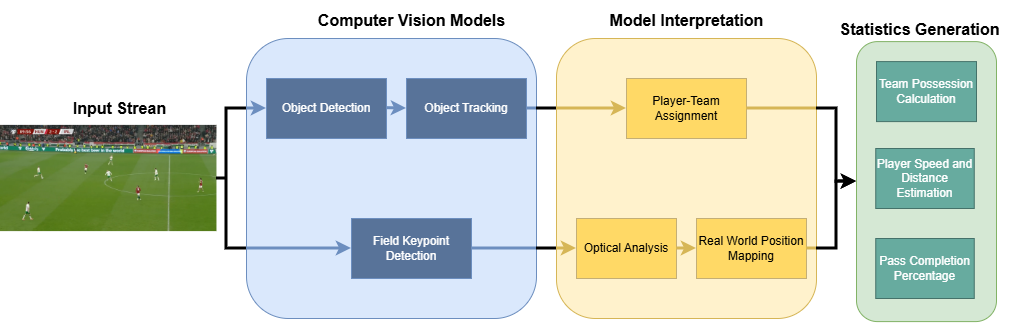
\includegraphics[width=\textwidth]{images/fulstack2.drawio.png}
  \caption{Proposed full-stack system diagram.}
  \label{fig:fullstack_system}
\end{figure}

Figure~\ref{fig:fullstack_system} illustrates how the trained object detection models, keypoint localisation models, and post-inference processing were integrated into the proposed full-stack system. Each video frame was processed both by an object detector and a pitch keypoint detector, with these intermediate outputs then consumed by the post-inference algorithms described previously. Inference could be performed either on every frame or at a configurable interval, to allow further hardware efficiency customisation. Confidence thresholds were applied to object detection, pitch keypoint detection, team-colour assignment, and pass classification.
